\documentclass[12pt]{article}
\title{Assignment 3: CS 754, Advanced Image Processing}
\author{\textbf{Group Details:} \\
Vinit Awale (18D070067)\\ 
Piyush Bharambe (18D070019)
}
\date{}
\usepackage{amsmath}
\usepackage{amssymb}
\usepackage{hyperref}
\usepackage{ulem}
\usepackage{enumitem}
\usepackage{float}
\usepackage{graphicx}
\usepackage{subcaption}
\usepackage{bm}
\pagenumbering{gobble}

\usepackage[margin=0.5in]{geometry}
\begin{document}
\maketitle
\begin{center}
    \section*{Question 1}
\end{center}

\begin{itemize}
    \item Your task here is to implement the ISTA algorithm for the following three cases:
\begin{enumerate}
\item Consider the image from the homework folder. Add iid Gaussian noise of mean 0 and variance 3 (on a [0,255] scale) to it, using the `randn' function in MATLAB. Thus $\boldsymbol{y} = \boldsymbol{x} + \boldsymbol{\eta}$ where $\boldsymbol{\eta} \sim \mathcal{N}(0,3)$ \textcolor{blue}{(earlier the variance was mistakenly marked as 4)}. You should obtain $\boldsymbol{x}$ from $\boldsymbol{y}$ using the fact that patches from $\boldsymbol{x}$ have a sparse or near-sparse representation in the 2D-DCT basis. 
\item Divide the image shared in the homework folder into patches of size $8 \times 8$. Let $\boldsymbol{x_i}$ be the vectorized version of the $i^{th}$ patch. Consider the measurement $\boldsymbol{y_i} = \boldsymbol{\Phi x_i}$ where $\boldsymbol{\Phi}$ is a $32 \times 64$ matrix with entries drawn iid from $\mathcal{N}(0,1)$. Note that $\boldsymbol{x_i}$ has a near-sparse representation in the 2D-DCT basis $\boldsymbol{U}$ which is computed in MATLAB as `kron(dctmtx(8)',dctmtx(8)')'. In other words, $\boldsymbol{x_i} = \boldsymbol{U \theta_i}$ where $\boldsymbol{\theta_i}$ is a near-sparse vector. Your job is to reconstruct each $\boldsymbol{x_i}$ given $\boldsymbol{y_i}$ and $\boldsymbol{\Phi}$ using ISTA. Then you should reconstruct the image by averaging the overlapping patches. You should choose the $\alpha$ parameter in the ISTA algorithm judiciously. Choose $\lambda = 1$ (for a [0,255] image). Display the reconstructed image in your report. State the RMSE given as $\|X(:)-\hat{X}(:)\|_2/\|X(:)\|_2$ where $\hat{X}$ is the reconstructed image and $X$ is the true image. \textsf{[15 points]}
\end{enumerate}
\textbf{Answer:}
\begin{enumerate}
    \item The original and the noisy (Gaussian Noise of standard deviation 3) Barbara images are shown below.
    \begin{figure}[H]
        \centering
        \begin{minipage}{.45\textwidth}
            \centering
            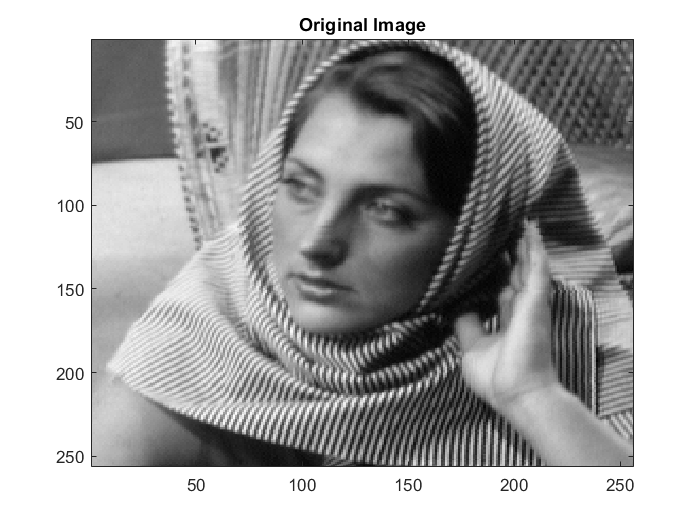
\includegraphics[width=\linewidth]{Images/Q1_Original.png}
            \caption*{Original Barbara Image}
        \end{minipage}
        \begin{minipage}{.55\textwidth}
            \centering
            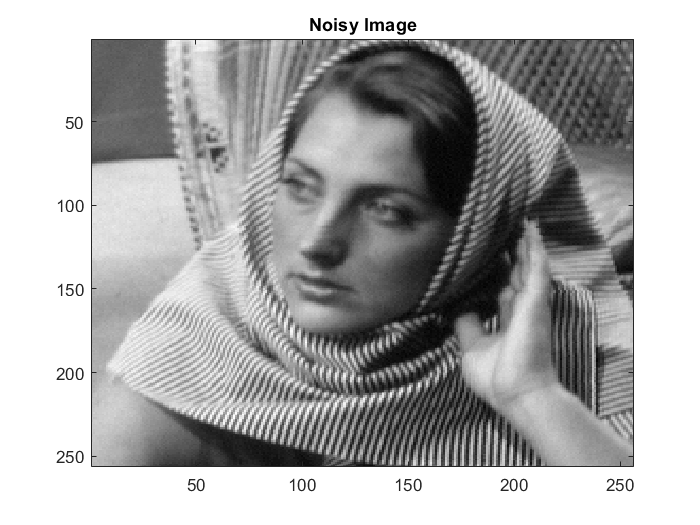
\includegraphics[width=\linewidth]{Images/Q1_Noisy.png}
            \caption*{Noisy Barbara Image}
        \end{minipage}
    \end{figure}
    
    \textbf{The RMSE between the original and the noisy image is $0.012663$}

     Now, we will use the noisy image as the input image and the original image as the ground truth. Using the input image and using the prior information that the patches in the ground truth image have a sparse representation in the 2D-DCT basis, we will reconstruct the image using ISTA algorithm. \\ 
     \textbf{Note:} In the ISTA algorithm, we have used $\lambda = 1$ and $\alpha = 1 + max(eigenvalue of A^TA)$ where $A$ is the measurement matrix. \\ 
     The reconstructed image using ISTA algorithm is as shown below. \\
    \begin{figure}[H]
        \centering
        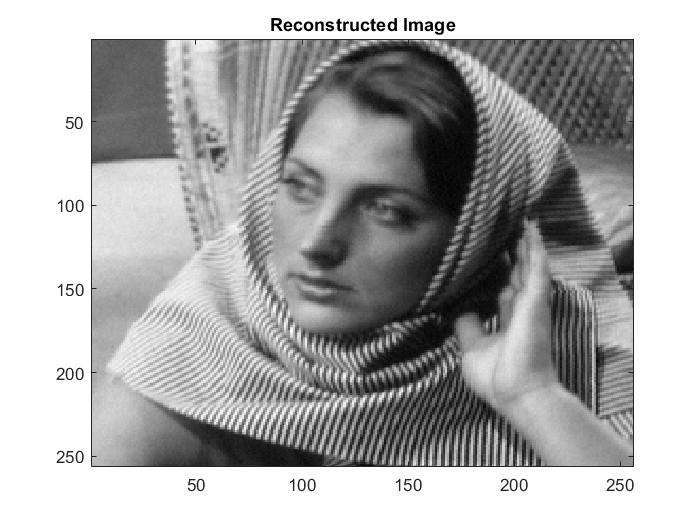
\includegraphics[width=0.55\linewidth]{Images/Q1_Part_a_result.png}
        \caption*{Reconstructed Image using ISTA}
    \end{figure}
    \textbf{The RMSE between the original and the reconstructed image using ISTA algorithm is $0.012366$}


    \item In this part, we consider 32 compressive measurements for each $8 \times 8$ patch. The entries of the measurement matrix are drawn iid from $\mathcal{N}(0,1)$. The ground truth image is the original Barbara image. We used ISTA algorithm on each overlapping patch and averaged the results. The reconstructed image is shown below. \\
    \textbf{Note:} This program takes roughly 124 seconds to run. \\
    \begin{figure}[H]
        \centering
        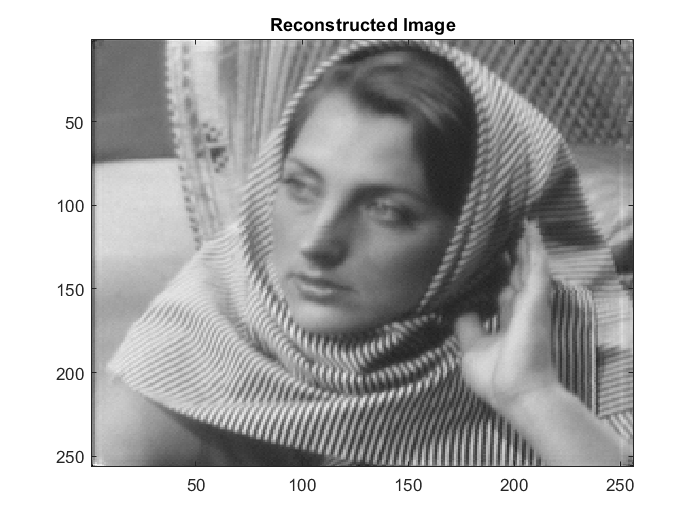
\includegraphics[width=0.55\linewidth]{Images/Q1_Part_b_result.png}
        \caption*{Reconstructed Image using ISTA on compressive measurements}
    \end{figure}
    \textbf{The RMSE between the original and the reconstructed image using ISTA algorithm on compressive measurements is $0.42538 $}

\end{enumerate}
\end{itemize}
\end{document}
